\documentclass[10pt,aspectratio=43]{beamer}
\usetheme{Berlin}

\usepackage{amsmath,bm,amsfonts,amssymb,enumerate,graphicx,animate,epsfig,bbm,calc,color,ifthen,capt-of,multimedia}
\usepackage{fancybox,xcolor,booktabs,colortbl}
\usepackage{physics}
\usepackage{../mycommand}%我惯用的命令,在本project中,存储在本文件的父文件夹
\graphicspath{{figures/}}

\usefonttheme{professionalfonts}
\usepackage[UTF8,fontset=none,scheme=chinese]{ctex}
\setmainfont{Times}
\setsansfont{Arial}
\setmonofont{Consolas}
\setCJKmainfont{SimSun}[BoldFont=SimHei,ItalicFont=KaiTi]
\setCJKsansfont{SimHei}
\setCJKmonofont{Microsoft YaHei}
\usepackage{unicode-math}
\setmathfont{XITS Math}

\usepackage{../beamercolorthemesustech}%效果同\usecolortheme{sustech},但\usecolortheme不支持自由选择文件路径,故调用底层的\usepackage命令
\definecolor{mygreen}{rgb}{0,0.6,0}
\definecolor{mymauve}{rgb}{0.58,0,0.82}
\definecolor{mygray}{gray}{.9}
\definecolor{mypink}{rgb}{.99,.91,.95}
\definecolor{mycyan}{cmyk}{.3,0,0,0}

\usepackage[ruled,linesnumbered]{algorithm2e}
\usepackage{verbatim,listings}
\lstset{ %
	backgroundcolor=\color{white},   % choose the background color
	basicstyle=\footnotesize\ttfamily,     % size of fonts used for the code
	columns=fullflexible,
	breaklines=true,                 % automatic line breaking only at whitespace
	captionpos=b,                    % sets the caption-position to bottom
	tabsize=4,
	commentstyle=\color{mygreen},    % comment style
	escapeinside={\%*}{*)},          % if you want to add LaTeX within your code
	keywordstyle=\color{blue},       % keyword style
	stringstyle=\color{mymauve}\ttfamily,     % string literal style
	numbers=left, 
	%	frame=single,
	rulesepcolor=\color{red!20!green!20!blue!20},
	% identifierstyle=\color{red},
	language=c
}

\setbeamertemplate{caption}[numbered]%添加图片的编号
\setbeamertemplate{sidebar right}{}%去掉默认添加的navigarion symbols
\setbeamercovered{transparent}%使未点出来的文字呈现透明,默认0.15透明度
\beamerdefaultoverlayspecification{}

%\usepackage[backend=biber,bibstyle=gb7714-2015,citestyle=verbose]{biblatex}
%\addbibresource{../reference.bib}

%题目,作者,学校,日期
\title{Boundedness and Stability}
\subtitle{\fontsize{9pt}{14pt}\textbf{第二次\quad SDEM 5.3}}
\author{杨徵羽}
%\institute{哈尔滨工业大学(威海)理学院}
\date{\today}

\begin{document}

\frame{\titlepage}

\begin{frame}[fragile]{markovianSwitching.m}
\begin{lstlisting}[language=matlab,
basicstyle=\ttfamily\scriptsize, 
numberstyle=\scriptsize]
function [rGrid] = markovianSwitching(Gamma, T, stepSize)
N = length(Gamma); % the quantity of states
iJump = 1; tJump(1) = 0; rJump(1) = randi(N); % initial value setting
while tJump(iJump) < T
      tJump(iJump+1) = tJump(iJump) + exprnd(-1/Gamma(rJump(iJump),rJump(iJump)));
      distribution = Gamma(rJump(iJump),:);
      distribution(rJump(iJump)) = 0;
      distribution = distribution/sum(distribution);
      rJump(iJump+1) = discretize(rand, cumsum([0 distribution]));
      iJump = iJump + 1;
end
%% convert to time grid in order to be compatible with numerical solutions
nJump = length(tJump);
tGrid = 0:stepSize:T; nGrid = length(tGrid); rGrid = zeros(1, nGrid);
tJumpGrid = ceil(tJump/stepSize);
for iJump = 1:nJump-1
    for iGrid = tJumpGrid(iJump)+1:tJumpGrid(iJump+1)
        rGrid(iGrid) = rJump(iJump);
    end
end
rGrid = rGrid(1:nGrid); % delete calculation beyond T
\end{lstlisting}
\end{frame}

\begin{frame}[fragile]{SDEMexample5\_4.m}
\begin{lstlisting}[language=matlab,
basicstyle=\ttfamily\scriptsize, 
numberstyle=\scriptsize]
clear;clc;close all;
nSample = 25; T = 20; stepSize = 0.01;
alpha = @(r)(1*(r==1)+(-1/2)*(r==2)); % a simple way of representing piecewise function
sigma = 5; gamma = 1.5; Gamma = [[-4 4]; [gamma -gamma]];
r = markovianSwitching(Gamma, T, stepSize); % one r(t) for all sample paths
tGrid = 0:stepSize:T;
nGrid = length(tGrid);
f = @(x,t,r) alpha(r) * x;
g = @(x,t,r) sigma;
x = zeros(nSample, nGrid); % not `zeros(nGrid)`!!!
for iSample = 1:nSample
    x(1) = 1;
    for iGrid = 1:nGrid - 1
        x(iSample, iGrid + 1) = x(iSample, iGrid) + f(x(iSample, iGrid), iGrid, r(iGrid)) * stepSize + g(x(iSample, iGrid), iGrid, r(iGrid)) * normrnd(0, stepSize);
    end
end
for iSample = 1:nSample
    plot(tGrid,x(iSample, :)); hold on
end
p = 2; pthmoment = mean(x.^p, 1);
plot(tGrid,pthmoment)
\end{lstlisting}
\end{frame}

\begin{frame}{全章结构}
\begin{table}[htbp]%\caption{全章结构}\label{t1}\centering
\resizebox{\columnwidth}{!}{
\begin{tabular}{cccccc}
\toprule
稳定性种类 & 节 & 定义 & V函数判别法 & 系数判别法 & 例子 \\
\midrule
p阶矩渐近有界 & 5.2 & 1 & 2 & 3 & 4,5 \\
p阶矩指数稳定 & 5.3 & 7 & 8 & 10,12,16 & 25,26,27 \\
p阶矩渐近稳定 & 5.4 & 28 & 29,30,31 &  & 32,33 \\
a.s.指数稳定 & 5.3 & 7 & 9 & 10,12,14,16 &  \\
a.s.渐近稳定 & 5.4 & 28 & 29 &  &  \\
依概率稳定 & 5.5 & 34 & 35 &  &  \\
依概率渐近稳定 & 5.5 & 34 & 36 &  & 38 \\
依概率渐近大范围稳定 & 5.5 & 34 & 37 &  &  \\
依分布渐近稳定 & 5.6 & 40 & 43 & 44 & 45,46 \\
\bottomrule
\end{tabular}
}
\end{table}
\end{frame}

\begin{frame}{5.3 Exponential Stability}
\begin{itemize}
\item Definition 5.7 p阶矩/a.s.指数稳定性定义
\item Lemma 5.1: 初值不为0 ↔ 解不为0(反证法,$ LV $计算,辅助函数$ e^{\lambda t}V $,含停时截断的It\^o公式)
\item Theorem 5.8: p阶矩指数稳定性V函数判别法(辅助函数$ e^{\lambda t}V $,含停时截断的It\^o公式)
\item Theorem 5.9: p阶矩指数稳定 → a.s.指数稳定(均值不等式,H\"older不等式,BDG不等式,Chebyshev-Borel-Cantelli三板斧)
\item Corollary 5.10: 系数判别法($ LV $计算,最大特征值)
\end{itemize}
\end{frame}

\begin{frame}{上次的$ LV $计算(SDEM p.159)}
\begin{figure}
\centering
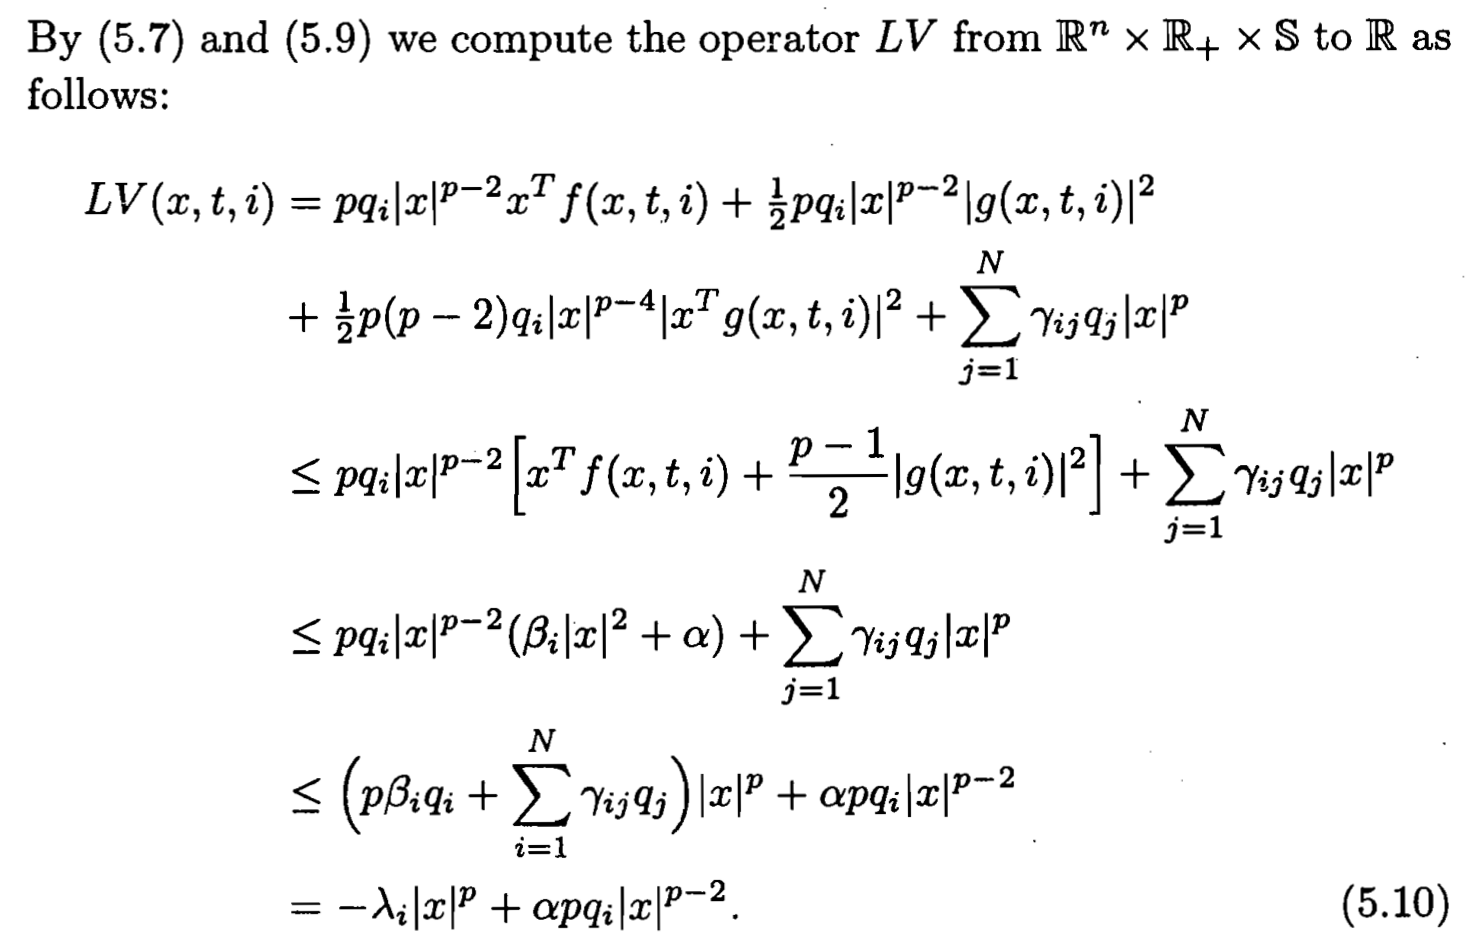
\includegraphics[width=\linewidth]{1}
\end{figure}
\end{frame}

\begin{frame}{BDG不等式(SDE p.127)}
\begin{figure}
\centering
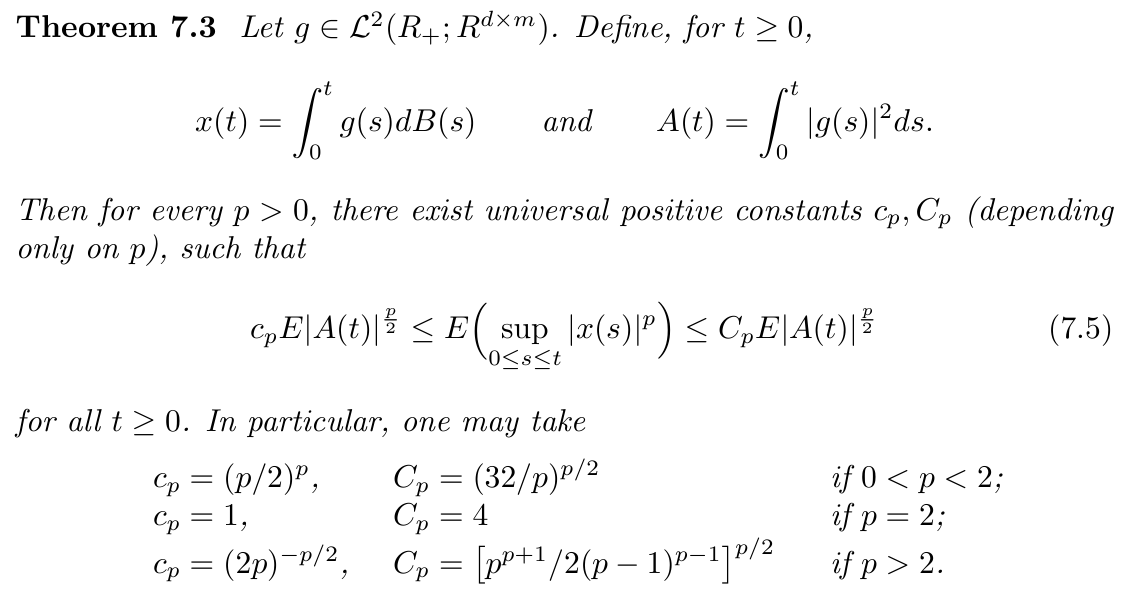
\includegraphics[width=\linewidth]{2}
\end{figure}
\end{frame}

\begin{frame}{Chebyshev不等式(SDEM p.7)}
\begin{figure}
\centering
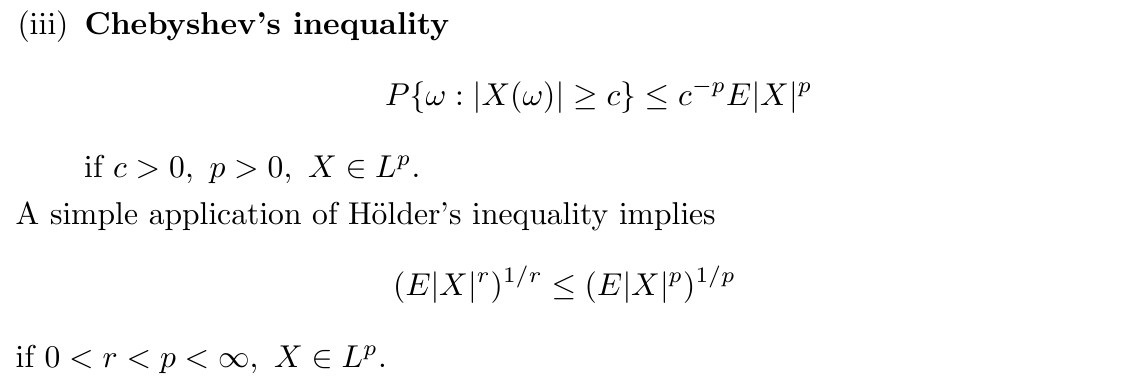
\includegraphics[width=\linewidth]{3}
\end{figure}
\end{frame}

\begin{frame}{Borel-Cantelli引理(SDEM p.10)}
\begin{figure}
\centering
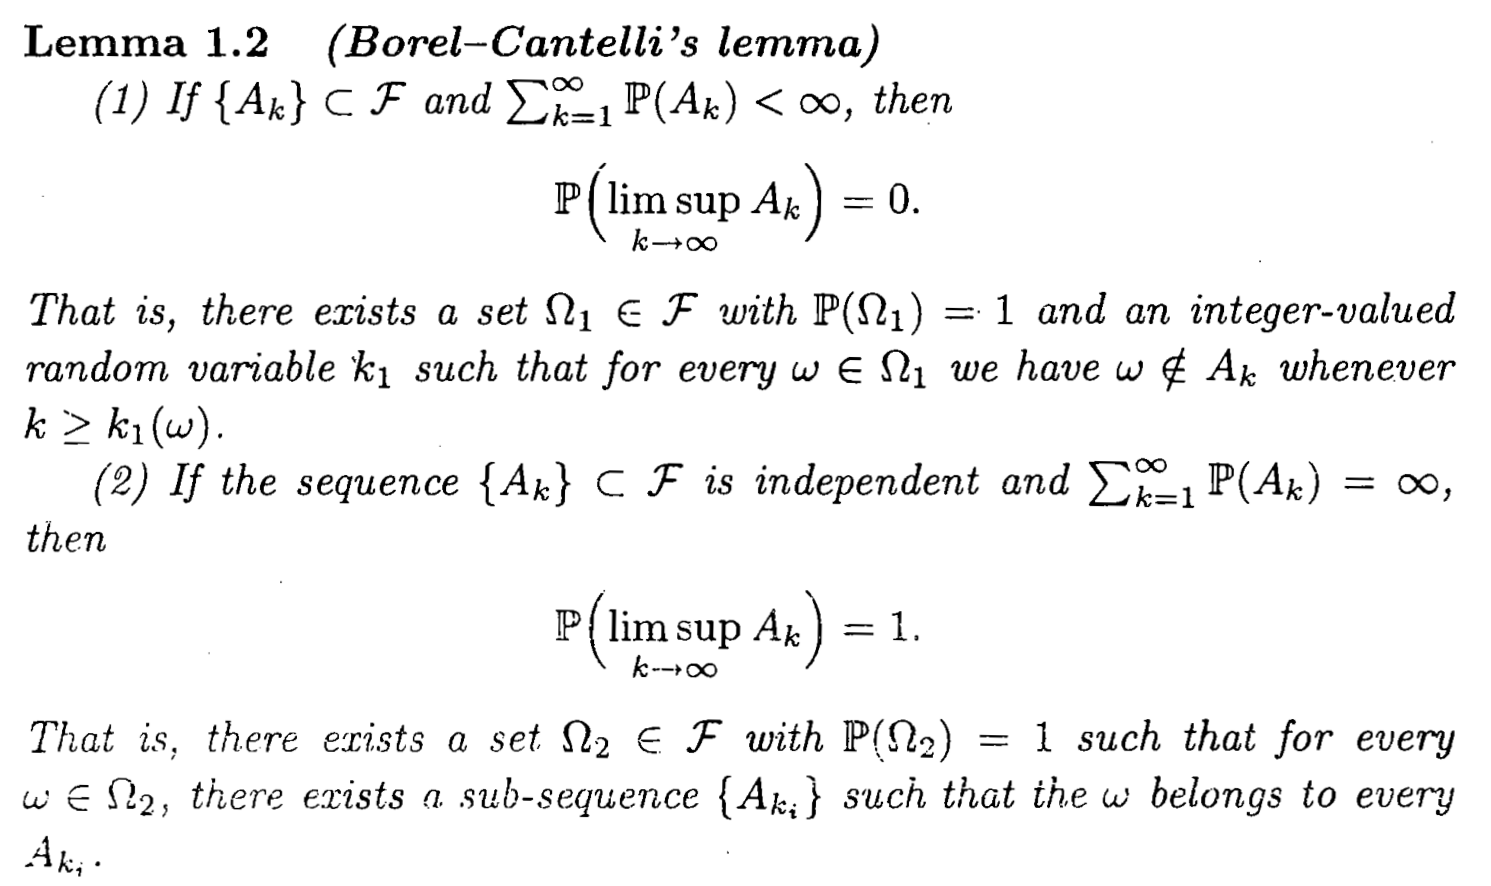
\includegraphics[width=\linewidth]{4}
\end{figure}
\end{frame}

\begin{frame}{最大/小特征值(SDEM p.59)}
\begin{figure}
\centering
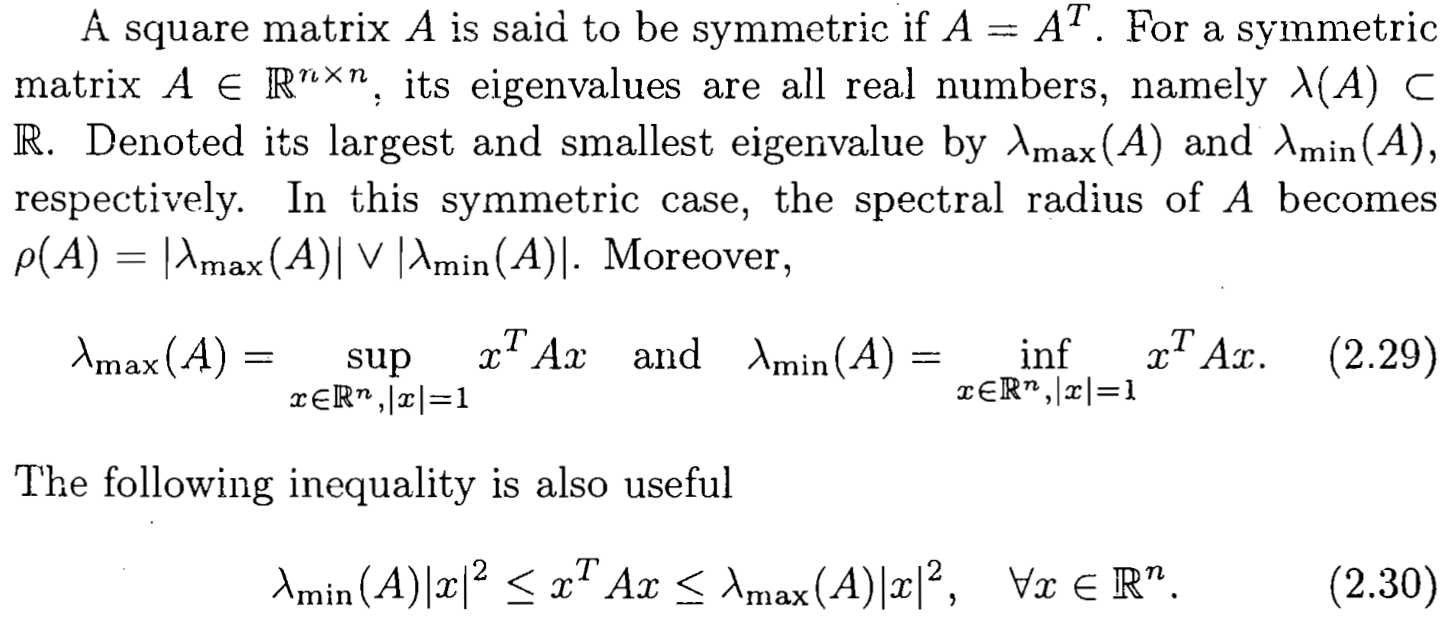
\includegraphics[width=\linewidth]{5}
\end{figure}
\end{frame}

\end{document}
